%\documentclass[11pt]{amsart}
\documentclass{article}
\usepackage{geometry}                % See geometry.pdf to learn the layout options. There are lots.
%\geometry{letterpaper}                   % ... or a4paper or a5paper or ... 
%\geometry{landscape}                % Activate for for rotated page geometry
%\usepackage[parfill]{parskip}    % Activate to begin paragraphs with an empty line rather than an indent
\usepackage{graphicx}
\usepackage{amssymb}
\usepackage{epstopdf}
\DeclareGraphicsRule{.tif}{png}{.png}{`convert #1 `dirname #1`/`basename #1 .tif`.png}
\title{Brief Article}
\author{The Author}
%\date{}                                           % Activate to display a given date or no date
%%%%%%%%%%%%%%%%%%
% SUMMARY OF USEFUL MACROS
%
% 1. \marginpar[LeftText]{RightText} Standard Latex \marginpar
%
% 2. \mymarginpar{MarginText}{BodyText} Places MarginText in margin and
%     BodyText in main text opposite margin. Places lineas above and below
%     text.  Used in element and model catalogs and elsewhere.
%
% 3. \marginlabel{text} Places large text in margin and underlines. Used
%    to put element name in margin at top of page for continued
%    descriptions.  Does not automaticly put it at the top of a page
%    and so a \clearpage is required.
%
% 4. \marginid{text} Used to place a short identifier in the margin. Just one
%    word and justified to the outside edge.
%
% 5. \offset a standard indent.
%
% 6. \offsetparbox{} Places text in an offset parbox.  Use
%    \hspace*{\fill} \offsetparbox{text}        to insert an offset text.
%
% 7. \boxed{} similar to above but starts a new line and right justifies
%    offsetparbox.
%
% 8. \form
%
% 9. \example
%
%10. \begin{widelist}  .... \end{widelist} 
%    A widelist that has 1 inch wide labels that has additional left hand
%    margin of 0.6 inch.
%
%11. \spicethreeonly{} Text is inserted only if output is for spice3.
%
%12. \pspiceonly{} 
%    Text is inserted only if output is for pspice (superspice for the most
%    part is upwards compatible to pspice).
%
%13. \sspiceonly{} 
%    Text is inserted only if output is for superspice but not for pspice.

%14. \sym{}
%    Right justifies a symbol in a keyword table.
%
%15. Use the following wherever as then we can have a standard way to
%    report them.  Note that "\dc\ " is required to get a space after dc.
%    \dc
%    \ac
%    \SPICE
%
%16. \kwnote{}  This is a convenient way to include notes in a keyword table.
%    It right justifies a note in the description column and starts it on a
%    newline.
\newcommand{\kwnote}[1]{\newline\hspace*{\fill} #1}

%
%17. \kwversion{} This is a convenient way to indicate versions in a keyword
%    table. It does a \kwnote .  It should not printed when outputing for
%     specific versions.
% typical usage is \kwversion{\sspice ; \hspice} to produce the output
%            VERSIONS: SUPERSPICE; HSPICE
% typical usage is \kwversionNote{\sspice ; \hspice} to produce the output
%                 |                    VERSIONS: SUPERSPICE; HSPICE |
%for unifomity the recommended version order is:
%    \hspice \pspice \sspice \spicetwo \spicethree
\newcommand{\version}[1]{({\sc version: #1})}
\newcommand{\kwversion}[1]{\newline({\sc version: #1})}
\newcommand{\kwversionNote}[1]{\kwnote{({\sc version: #1})}}
\newcommand{\versions}[1]{({\sc versions: #1})}
\newcommand{\kwversions}[1]{\newline({\sc versions: #1})}
\newcommand{\kwversionsNote}[1]{\kwnote{({\sc versions: #1})}}

%


\newcommand{\mymargin}{1in}   % Use to set width of margin notes
\newcommand{\mymarginparsep}{0.1in}
\newcommand{\mymarginparsepplustext}{5.6in}
\newcommand{\mymarginplus}{1.1in}
\newcommand{\mymarginplustext}{6.6in}
\newcommand{\underlinehead}{\\[-0.1in] \rule{\mymarginplustext}{0.01in}}
\newcommand{\overlinefoot}{\rule{\mymarginplustext}{0.01in}\\}
% WIDEPARBOX uses margin space as well.
\newcommand{\wideparbox}[1]{\parbox[t]{\mymarginplustext}{#1}}
%
% HEADER AND FOOT
% Standard header and foot, but includes copyright notice.a
% To omit copyrite notice do not include copyrite.sty
%
\newcommand{\mycopyrite}{}
\def\ps@headings{\let\@mkboth\markboth
\def\@oddfoot{\wideparbox{\overlinefoot\rm\today \hfill \mycopyrite}}
\def\@evenfoot{\hspace*{-\mymarginplus}\wideparbox{\overlinefoot
\mycopyrite\hfill \today}}
\def\@evenhead{\hspace*{-\mymarginplus}\wideparbox{\rm
\thepage\hfill \sl \leftmark \underlinehead }}
\def\@oddhead{\wideparbox{\hbox{}\sl \rightmark \hfill
\rm\thepage \underlinehead}}\def\chaptermark##1{\markboth {\uppercase{\ifnum
\c@secnumdepth
>\m@ne
 \@chapapp\ \thechapter. \ \fi ##1}}{}}\def\sectionmark##1{\markright
 {\uppercase{\ifnum \c@secnumdepth >\z@
  \thesection. \ \fi ##1}}}}

%\oddsidemargin 0.25in \topmargin 0.0in \textwidth 6.5in \textheight 9in
%\evensidemargin 0.25in \headheight 0.18in \footskip 0.16in

%%   EPSF.TEX macro file:
%   Written by Tomas Rokicki of Radical Eye Software, 29 Mar 1989.
%   Revised by Don Knuth, 3 Jan 1990.
%   Revised by Tomas Rokicki to accept bounding boxes with no
%      space after the colon, 18 Jul 1990.
%
%   TeX macros to include an Encapsulated PostScript graphic.
%   Works by finding the bounding box comment,
%   calculating the correct scale values, and inserting a vbox
%   of the appropriate size at the current position in the TeX document.
%
%   To use with the center environment of LaTeX, preface the \epsffile
%   call with a \leavevmode.  (LaTeX should probably supply this itself
%   for the center environment.)
%
%   To use, simply say
%   \input epsf           % somewhere early on in your TeX file
%   \epsfbox{filename.ps} % where you want to insert a vbox for a figure
%
%   Alternatively, you can type
%
%   \epsfbox[0 0 30 50]{filename.ps} % to supply your own BB
%
%   which will not read in the file, and will instead use the bounding
%   box you specify.
%
%   The effect will be to typeset the figure as a TeX box, at the
%   point of your \epsfbox command. By default, the graphic will have its
%   `natural' width (namely the width of its bounding box, as described
%   in filename.ps). The TeX box will have depth zero.
%
%   You can enlarge or reduce the figure by saying
%     \epsfxsize=<dimen> \epsfbox{filename.ps}
%   (or
%     \epsfysize=<dimen> \epsfbox{filename.ps})
%   instead. Then the width of the TeX box will be \epsfxsize and its
%   height will be scaled proportionately (or the height will be
%   \epsfysize and its width will be scaled proportiontally).  The
%   width (and height) is restored to zero after each use.
%
%   A more general facility for sizing is available by defining the
%   \epsfsize macro.    Normally you can redefine this macro
%   to do almost anything.  The first parameter is the natural x size of
%   the PostScript graphic, the second parameter is the natural y size
%   of the PostScript graphic.  It must return the xsize to use, or 0 if
%   natural scaling is to be used.  Common uses include:
%
%      \epsfxsize  % just leave the old value alone
%      0pt         % use the natural sizes
%      #1          % use the natural sizes
%      \hsize      % scale to full width
%      0.5#1       % scale to 50% of natural size
%      \ifnum#1>\hsize\hsize\else#1\fi  % smaller of natural, hsize
%
%   If you want TeX to report the size of the figure (as a message
%   on your terminal when it processes each figure), say `\epsfverbosetrue'.
%
\newread\epsffilein    % file to \read
\newif\ifepsffileok    % continue looking for the bounding box?
\newif\ifepsfbbfound   % success?
\newif\ifepsfverbose   % report what you're making?
\newdimen\epsfxsize    % horizontal size after scaling
\newdimen\epsfysize    % vertical size after scaling
\newdimen\epsftsize    % horizontal size before scaling
\newdimen\epsfrsize    % vertical size before scaling
\newdimen\epsftmp      % register for arithmetic manipulation
\newdimen\pspoints     % conversion factor
%
\pspoints=1bp          % Adobe points are `big'
\epsfxsize=0pt         % Default value, means `use natural size'
\epsfysize=0pt         % ditto
%
\def\epsfbox#1{\global\def\epsfllx{72}\global\def\epsflly{72}%
   \global\def\epsfurx{540}\global\def\epsfury{720}%
   \def\lbracket{[}\def\testit{#1}\ifx\testit\lbracket
   \let\next=\epsfgetlitbb\else\let\next=\epsfnormal\fi\next{#1}}%
%
\def\epsfgetlitbb#1#2 #3 #4 #5]#6{\epsfgrab #2 #3 #4 #5 .\\%
   \epsfsetgraph{#6}}%
%
\def\epsfnormal#1{\epsfgetbb{#1}\epsfsetgraph{#1}}%
%
\def\epsfgetbb#1{%
%
%   The first thing we need to do is to open the
%   PostScript file, if possible.
%
\openin\epsffilein=#1
\ifeof\epsffilein\errmessage{I couldn't open #1, will ignore it}\else
%
%   Okay, we got it. Now we'll scan lines until we find one that doesn't
%   start with %. We're looking for the bounding box comment.
%
   {\epsffileoktrue \chardef\other=12
    \def\do##1{\catcode`##1=\other}\dospecials \catcode`\ =10
    \loop
       \read\epsffilein to \epsffileline
       \ifeof\epsffilein\epsffileokfalse\else
%
%   We check to see if the first character is a % sign;
%   if not, we stop reading (unless the line was entirely blank);
%   if so, we look further and stop only if the line begins with
%   `%%BoundingBox:'.
%
          \expandafter\epsfaux\epsffileline:. \\%
       \fi
   \ifepsffileok\repeat
   \ifepsfbbfound\else
    \ifepsfverbose\message{No bounding box comment in #1; using defaults}\fi\fi
   }\closein\epsffilein\fi}%
%
%   Now we have to calculate the scale and offset values to use.
%   First we compute the natural sizes.
%
\def\epsfclipstring{}% do we clip or not?  If so,
\def\epsfclipon{\def\epsfclipstring{ clip}}%
\def\epsfclipoff{\def\epsfclipstring{}}%
%
\def\epsfsetgraph#1{%
   \epsfrsize=\epsfury\pspoints
   \advance\epsfrsize by-\epsflly\pspoints
   \epsftsize=\epsfurx\pspoints
   \advance\epsftsize by-\epsfllx\pspoints
%
%   If `epsfxsize' is 0, we default to the natural size of the picture.
%   Otherwise we scale the graph to be \epsfxsize wide.
%
   \epsfxsize\epsfsize\epsftsize\epsfrsize
   \ifnum\epsfxsize=0 \ifnum\epsfysize=0
      \epsfxsize=\epsftsize \epsfysize=\epsfrsize
      \epsfrsize=0pt
%
%   We have a sticky problem here:  TeX doesn't do floating point arithmetic!
%   Our goal is to compute y = rx/t. The following loop does this reasonably
%   fast, with an error of at most about 16 sp (about 1/4000 pt).
% 
     \else\epsftmp=\epsftsize \divide\epsftmp\epsfrsize
       \epsfxsize=\epsfysize \multiply\epsfxsize\epsftmp
       \multiply\epsftmp\epsfrsize \advance\epsftsize-\epsftmp
       \epsftmp=\epsfysize
       \loop \advance\epsftsize\epsftsize \divide\epsftmp 2
       \ifnum\epsftmp>0
          \ifnum\epsftsize<\epsfrsize\else
             \advance\epsftsize-\epsfrsize \advance\epsfxsize\epsftmp \fi
       \repeat
       \epsfrsize=0pt
     \fi
   \else \ifnum\epsfysize=0
     \epsftmp=\epsfrsize \divide\epsftmp\epsftsize
     \epsfysize=\epsfxsize \multiply\epsfysize\epsftmp   
     \multiply\epsftmp\epsftsize \advance\epsfrsize-\epsftmp
     \epsftmp=\epsfxsize
     \loop \advance\epsfrsize\epsfrsize \divide\epsftmp 2
     \ifnum\epsftmp>0
        \ifnum\epsfrsize<\epsftsize\else
           \advance\epsfrsize-\epsftsize \advance\epsfysize\epsftmp \fi
     \repeat
     \epsfrsize=0pt
    \else
     \epsfrsize=\epsfysize
    \fi
   \fi
%
%  Finally, we make the vbox and stick in a \special that dvips can parse.
%
   \ifepsfverbose\message{#1: width=\the\epsfxsize, height=\the\epsfysize}\fi
   \epsftmp=10\epsfxsize \divide\epsftmp\pspoints
   \vbox to\epsfysize{\vfil\hbox to\epsfxsize{%
      \ifnum\epsfrsize=0\relax
        \special{PSfile=#1 llx=\epsfllx\space lly=\epsflly\space
            urx=\epsfurx\space ury=\epsfury\space rwi=\number\epsftmp
            \epsfclipstring}%
      \else
        \epsfrsize=10\epsfysize \divide\epsfrsize\pspoints
        \special{PSfile=#1 llx=\epsfllx\space lly=\epsflly\space
            urx=\epsfurx\space ury=\epsfury\space rwi=\number\epsftmp\space
            rhi=\number\epsfrsize \epsfclipstring}%
      \fi
      \hfil}}%
\global\epsfxsize=0pt\global\epsfysize=0pt}%
%
%   We still need to define the tricky \epsfaux macro. This requires
%   a couple of magic constants for comparison purposes.
%
{\catcode`\%=12 \global\let\epsfpercent=%\global\def\epsfbblit{%BoundingBox}}%
%
%   So we're ready to check for `%BoundingBox:' and to grab the
%   values if they are found.
%
\long\def\epsfaux#1#2:#3\\{\ifx#1\epsfpercent
   \def\testit{#2}\ifx\testit\epsfbblit
      \epsfgrab #3 . . . \\%
      \epsffileokfalse
      \global\epsfbbfoundtrue
   \fi\else\ifx#1\par\else\epsffileokfalse\fi\fi}%
%
%   Here we grab the values and stuff them in the appropriate definitions.
%
\def\epsfempty{}%
\def\epsfgrab #1 #2 #3 #4 #5\\{%
\global\def\epsfllx{#1}\ifx\epsfllx\epsfempty
      \epsfgrab #2 #3 #4 #5 .\\\else
   \global\def\epsflly{#2}%
   \global\def\epsfurx{#3}\global\def\epsfury{#4}\fi}%
%
%   We default the epsfsize macro.
%
\def\epsfsize#1#2{\epsfxsize}
%
%   Finally, another definition for compatibility with older macros.
%
\let\epsffile=\epsfbox

\usepackage{epsf}
\oddsidemargin 0.25in \evensidemargin 0.25in
\topmargin 0.0in
\textwidth 6.5in \textheight 9in
\headheight 0.18in \footskip 0.16in
\leftmargin -0.5in \rightmargin -0.5in

\newcommand{\fig}[1]{figures/#1}
\newcommand{\pfig}[1]{\epsfbox{\fig{#1}}}
\newcommand{\newfig}[1]{\epsffile{\fig{#1}}}

\newcommand{\fdaelement}[1]{elements/#1}
\newcommand{\spiceelement}[1]{equivalent_spice_elements/#1}

\newcommand{\FREEDA}{{\Huge{\textsl{\textsf{f}}}${\mathsf{REEDA}}^{{\tiny{\textsf{TM}}}}$}}
\newcommand{\FDA}{{\textsl{\textsf{f}}}${\mathsf{REEDA}}^{{\tiny{\textsf{TM}}}}$}
\newcommand{\notforsspice}[1]{#1}
\newcommand{\spicetwoonly}[1]{#1}
\newcommand{\spicethreeonly}[1]{#1}
\newcommand{\pspiceonly}[1]{#1}
\newcommand{\pspiceninetytwoonly}[1]{#1}
\newcommand{\sspiceonly}[1]{}
\newcommand{\fornutmeg}[1]{}
\newcommand{\sspicetwoonly}[1]{}

%%%%%%%%%%%%%%%%%%%%%%%%%%%%%%%%%%%%%%%%%%%%%%%%%%%%%%%%%%%%%%%%%%%%%%%%%%%%%%%%
\marginparwidth=\mymargin
\marginparsep=\mymarginparsep
\newcommand{\textplusmarginparwidth}{\textwidth+\marginparsep+\mymargin}
\newcommand{\X}{\\ \hline}    % line terminataion in keyword environment
\newcommand{\B}{{ \rm [}}     % begin optional parameter in \form{}
\newcommand{\E}{{\ \rm\hspace{-0.04in}] }}   % end optional parameter in \form{}
\newcommand{\expr}{{\sc Expressions supported}}
\newcommand{\reqd}{{\scriptsize REQUIRED}}
\newcommand{\omitted}{{\scriptsize OMITTED}}
\newcommand{\inferred}{{\scriptsize INFERRED}}
\newcommand{\para}{\newline{\scriptsize (PARASITIC)}}
\newcommand{\opt}{{\tiny  OPTIONAL}}

\newcommand{\Spice}{{\sc Spice}}
\newcommand{\spice}{{\sc Spice}}
\newcommand{\justspice}{{\sc Spice}}
\newcommand{\nutmeg}{{\sc NUTMEG}}
\newcommand{\probe}{{\sc Probe}}

\newcommand{\accusim}{{\sc AccuSim}}
\newcommand{\contec}{{\sc ContecSpice}}
\newcommand{\cdsspice}{{\sc CDS Spice}}
\newcommand{\hpimpulse}{{\sc HP Impulse}}
\newcommand{\hspice}{{\sc HSpice}}
\newcommand{\igspice}{{\sc IG\_SPICE}}
\newcommand{\isspice}{{\sc IsSpice}}
\newcommand{\mspice}{{\sc Microwave Spice}}
\newcommand{\pspice}{{\sc PSpice}}
\newcommand{\justpspice}{{\sc PSpice}}
\newcommand{\spectre}{{\sc Spectre}}
\newcommand{\spicetwo}{{\sc Spice2g6}}
\newcommand{\spicethree}{{\sc Spice3}}
\newcommand{\spiceplus}{{\sc SpicePlus}}
\newcommand{\sspice}{{\sc SuperSpice}}

\newcommand{\modelversion}[1]{& #1}
%%%%%%%%%%%%%%%%%%%%%%%%%%%%%%%%%%%%%%%%%%%%%%%%%%%%%%%%%%%%%%%%%%%%%%%%%%%%%%%%
% set up a counter for all occasions
%
\newcounter{count}

% set up new commands
%
\newcommand{\vshift}{\vspace{0.2in}}
% OFFSET
\newcommand{\offset}{\hspace*{0.45in} }
% OFFSETPARBOXWIDTH argument should be \textwith - offset
\newcommand{\offsetparbox}[1]{\parbox[t]{5in}{#1}}

% note: no labeling
\newcommand{\elementx}[3]{\clearpage\rm\markright{#3:#2}
\addcontentsline{toc}{section}{#1, #2: #3}
\mymarginparx{#1}{#2}{#3}\index{#1:#2}\index{#3:#2}}

% macros for sub elements
\newcommand{\subelement}[2]{\clearpage 
   \noindent\rule{\textwidth /2}{.5mm} \\[0.1in]
   {\large \bf #1} \hspace{0.2in} {\bf #2} \\
   \noindent\rule{\textwidth /2}{.5mm} \index{#1} \index{#2}}
% macros for models
\newcommand{\model}[2]{{
   \noindent\vspace{0.2in}\parbox{\textwidth}{
   \noindent\rule{\textwidth}{.5mm} \\[0.1in]
   {\large \bf #1 Model} \label{#1model} \hfill {\large #2} \\
   \noindent\rule{\textwidth}{.5mm} \index{#1} \index{#2}}}}
\newcommand{\modelx}[3]{{
   \noindent\vspace{0.2in}\parbox{\textwidth}{
   \noindent\rule{\textwidth}{.5mm} \\[0.1in]
   {\large \bf #1 Model} \hfill {\large #2} \hfill {\large #3} \\
   \noindent\rule{\textwidth}{.5mm} \index{#1} \index{#2}}}}



% BOXED
\newcommand{\boxed}[1]{\noindent
\newline \vshift \hspace*{\fill} {\tt \offsetparbox{\tt #1}}
 \vshift}


%
% KEYWORD
%
\newcommand{\keywordtable}[1]{
        \sloppy
        \hyphenation{ca-pac-i-t-an-ce} 
        \begin{center}
    \sf
        \begin{tabular}[t]
        {|p{0.58in}|p{3.07in}|p{0.55in}|p{0.60in}|}
        \hline
        \multicolumn{1}{|c}{\bf Name} &
        \multicolumn{1}{|c}{\parbox{2.77in}{\bf Description}}  &
        \multicolumn{1}{|c}{\bf Units} &
        \multicolumn{1}{|c|}{\bf Default} \X
        #1
        \end{tabular}
        \end{center}
    }

\newcommand{\keywordtwotable}[2]{
        \sloppy
        \hyphenation{ca-pac-i-t-an-ce} 
        \begin{center}
    \sf
        \begin{tabular}[t]
        {|p{0.58in}|p{2.38in}|p{0.55in}|p{0.60in}|p{0.53in}|}
        \hline
        \multicolumn{1}{|c}{\bf Name} &
        \multicolumn{1}{|c}{\parbox{2.20in}{\bf Description}}  &
        \multicolumn{1}{|c}{\bf Units} &
        \multicolumn{1}{|c}{\bf Default} &
        \multicolumn{1}{|c|}{\bf #1} \X
        #2
        \end{tabular}
        \end{center}
    }

\newcommand{\kw}[2]{
     \samepage{
     \noindent {\sl #1} \vspace{-0.5in} \\
     \keywordtable{#2} }}

\newcommand{\kwtwo}[3]{
     \samepage{
     \noindent {\sl #1} \vspace{-0.4in} \\
     \keywordtwotable{#2}{#3} }}

\newcommand{\keyword}[1]{\kw{Keywords:}{#1}}
\newcommand{\keywordtwo}[2]{\kwtwo{Keywords:}{#1}{#2}}
\newcommand{\modelkeyword}[1]{\kw{Model Keywords}{#1}}
\newcommand{\modelkeywordtwo}[2]{\kwtwo{Model Keywords}{#1}{#2}}

\newcommand{\myline}{\\[-0.1in]
\noindent \rule{\textwidth}{0.01in} \newline}

\newcommand{\myThickLine}{\\[-0.1in]
\noindent \rule{\textwidth}{0.02in} \newline}


% SPICE 2G6 FORM
%\newcommand{\spicetwoform}[1]{
%\spicetwoonly{\samepage{\noindent{\sl\spicetwo\form{#1}}}}}

% PSPICE88 FORM
%\newcommand{\pspiceform}[1]{
%\pspiceonly{\samepage{\noindent{\sl\pspice}\form{#1}}}}

% PSPICE92 FORM
%\newcommand{\pspiceninetytwoform}[1]{
%\pspiceninetytwoonly{\samepage{\noindent{\sl\pspice92\form{#1}}}}}


% SPICE3E2 FORM
%\newcommand{\spicethreeform}[1]{
%\spicethreeonly{\samepage{\noindent{\sl\spicethree\form{#1}}}}}

% FORM
\newcommand{\form}[1]{\samepage{\noindent
 {\sl Form} \myline
% \hspace*{\fill} % For some reason \fill = 0 when \pspiceform{} is used?
\offset
\it  \offsetparbox{#1}}
\\[0.1in]}

% ELEMENT FORM
\newcommand{\elementform}[1]{\samepage{\noindent
 {\sl Element Form} \myline
% \hspace*{\fill} % For some reason \fill = 0 when \pspiceform{} is used?
\offset
\it  \offsetparbox{#1}}
\\[0.1in]}

% MODEL FORM
\newcommand{\modelform}[1]{\samepage{\noindent
 {\sl Model Form} \myline
% \hspace*{\fill} % For some reason \fill = 0 when \pspiceform{} is used?
\offset
\it  \offsetparbox{#1}}
\\[0.1in]}

% LIMITS
\newcommand{\mylimits}[1]{\samepage{\noindent
 {\sl Limits} \myline
 \hspace*{\fill} \it  \offsetparbox{#1}}
 \vshift}

% EXAMPLE
\newcommand{\example}[1]{\samepage{\noindent
{\sl Example} \myline
\offset \tt  \offsetparbox{#1}}
 \vshift}

% PSPICE88 EXAMPLE
\newcommand{\pspiceexample}[1]{\samepage{\noindent
{\sl \pspice\ Example} \myline
\offset \tt  \offsetparbox{#1}}
 \vshift}

% MODEL TYPES
\newcommand{\modeltype}[1]{\samepage{\noindent
{\sl Model Type} \myline
 \hspace*{\fill} \tt \offsetparbox{#1}}
 \\[0.1in]}

% MODEL TYPES
\newcommand{\modeltypes}[1]{\samepage{\noindent
{\sl Model Types:} \myline
 \hspace*{\fill} \tt \offsetparbox{\tt #1}}
 \vshift}

% OFFSET ENUMERATE
\newcommand{\offsetenumerate}[1]{
     \offset \hspace*{-0.1in} {\begin{enumerate} #1 \end{enumerate}}}

% NOTE
\newcommand{\note}[1]{
\vshift\samepage{\noindent {\sl Note}\myline\vspace{-0.24in}}
 \offsetenumerate{#1} }

% SPECIAL NOTE
\newcommand{\specialnote}[2]{
\vshift\samepage{\noindent {\sl #1}\myline\vspace{-0.24in}}\\#2}

\newcommand{\dc}{\mbox{\tt DC}}
\newcommand{\ac}{\mbox{\tt AC}}
\newcommand{\SPICE}{\mbox{\tt SPICE}}
\newcommand{\m}[1]{{\bf #1}}                           % matrix command  \m{}

% ////// Changing nodes to terminals///////
% print terminals in \tt and enclose in a circle use outside
\newcommand{\terminal}[1]{\: \mbox{\tt #1} \!\!\!\! \bigcirc }
%
% set up environment for example
%
\newcounter{excount}
\newcounter{dummy}
\newenvironment{eg}{\vspace{0.1in}\noindent\rule{\textwidth}{.5mm}
   \begin{list}
   {{\addtocounter{excount}{1}
   \em Example\/ \arabic{chapter}.\arabic{excount}\/}:}
   {\usecounter{dummy}
   \setlength{\rightmargin}{\leftmargin}}
   }{\end{list} \rule{\textwidth}{.5mm}\vspace{0.1in}}
%
% set up environment for block
% currently this draws a horizontal line at the start of block and another
% at the end of block.
%
\newenvironment{block}{\vspace{0.1in}\noindent\rule{\textwidth}{.5mm}
   }{\rule{\textwidth}{.5mm}\vspace{0.1in}}
%

%
% Macros for element summaries
%
% macros for element summary
%\newcommand{\summaryelement}[2]{
%   \vspace{0.4in}
%   \mymarginpar{#1}{#2} 
%   \addcontentsline{toc}{section}{#1, #2}
%   \vspace{-0.6in} \\
%   \noindent Full description on page \pageref{#1element}. \vshift\\
%   }

% Summary MODEL TYPE
%\newcommand{\summarymodeltype}[1]{\samepage{\noindent
%{\sl Model Type} \myline
% \hspace*{\fill} \tt \offsetparbox{\tt #1
% \hfill Summary on \pageref{#1summary} \index{#1}}}
% }

% Summary MODEL TYPES
%\newcommand{\summarymodeltypes}[1]{\samepage{\noindent
%{\sl Model Types} \myline
% \hspace*{\fill} \tt \offsetparbox{\tt #1
% \hfill Summary on \pageref{#1summary} \index{#1}}}
% }

%
% macros for model summary
%\newcommand{\summarymodel}[2]{\clearpage
%   \addcontentsline{toc}{section}{#1, #2}
%   \mymarginpar{#1}{#2} \label{#1summary}
%   \index{#1} \index{#2}
%   \noindent Full description on page \pageref{#1model} \\[0.1in]
%   }



%
% set up wide descriptive list
%
\newenvironment{widelist}
    {\begin{list}{}{\setlength{\rightmargin}{0in} \setlength{\itemsep}{0.1in}
    \setlength{\labelwidth}{0.95in} \setlength{\labelsep}{0.1in}
\setlength{\listparindent}{0in} \setlength{\parsep}{0in}
    \setlength{\leftmargin}{1.0in}}
    }{\end{list}}

\newcommand{\STAR}{\hspace*{\fill} * \hspace*{\fill}}

\newcommand{\sym}[1]{\hspace*{\fill} ($#1$)}

%
% The thebibliography environment is redefined so the the word References is
% not output
%\def\thebibliography#1{\list
% {[\arabic{enumi}]}{\settowidth\labelwidth{[#1]}\leftmargin\labelwidth
% \advance\leftmargin\labelsep
% \usecounter{enumi}}
% \def\newblock{\hskip .11em plus .33em minus -.07em}
% \sloppy\clubpenalty4000\widowpenalty4000
% \sfcode`\.=1000\relax}
%\let\endthebibliography=\endlist
% END thebibliography environment redefinition



%\newcommand{\eskipv}[1]{\clearpage\marginlabel{#1}}
%\newcommand{\eskip}[1]{\vspace*{\fill}\clearpage\marginlabel{#1}}
%\newcommand{\eskipnv}[1]{\newpage\marginlabel{#1}}
%\newcommand{\eskipn}[1]{\vspace*{\fill}\newpage\marginlabel{#1}}

%marginlabel is very wide
%\newcommand{\eskipfullv}[1]{\clearpage\marginlabelfull{#1}}
%\newcommand{\eskipfull}[1]{\vspace*{\fill}\clearpage\marginlabelfull{#1}}
%\newcommand{\eskipfullnv}[1]{\newpage\marginlabelfull{#1}}
%\newcommand{\eskipfulln}[1]{\vspace*{\fill}\newpage\marginlabelfull{#1}}

%\newcommand{\mycontentsline}[5]{\parbox{#1}{#2}#3
%\hspace{0.1in}\dotfill\parbox{0.3in}{\hfill\pageref{#4#5}}\\[0.1in]}
%\newcommand{\mysline}[2]{\mycontentsline{1.2in}{#1}{#2}{#1}{statement}}
%\newcommand{\mymline}[2]{\mycontentsline{0.7in}{#1}{#2}{#1}{model}}
%\newcommand{\myeline}[2]{\mycontentsline{0.7in}{#1}{#2}{#1}{element}}

%\newcommand{\myincontentsline}[5]{\vspace{0.05in}\noindent\parbox{#1}{#2}#3
%\hspace{0.1in}
%\dotfill\parbox{0.7in}{\hfill Page \pageref{#4#5}}\\[0.05in]\noindent}
%\newcommand{\myinsline}[2]{\myincontentsline{1.2in}{#1}{#2}{#1}{statement}}
%\newcommand{\myinmline}[2]{\myincontentsline{0.5in}{#1}{#2}{#1}{model}}
%\newcommand{\myineline}[2]{\myincontentsline{0.5in}{#1}{#2}{#1}{element}}

%
%
% The following a symbols that could used alot.
\newcommand{\ms}[1]{\mbox{\scriptsize #1}}
\newcommand{\AF}{A_F}
\newcommand{\CBD}{C'_{BD}}
\newcommand{\CBS}{C'_{BS}}
\newcommand{\CGBO}{C_{GBO}}
\newcommand{\CGDO}{C_{GDO}}
\newcommand{\CGSO}{C_{GSO}}
\newcommand{\CJ}{C_J}
\newcommand{\CJSW}{C_{J,\ms{SW}}}
\newcommand{\DELTA}{\delta}
\newcommand{\ETA}{\eta}
\newcommand{\FC}{F_C}
\newcommand{\GAMMA}{\gamma}
\newcommand{\IS}{I_S}
\newcommand{\JS}{J_S}
\newcommand{\KAPPA}{\kappa}
\newcommand{\KF}{K_F}
\newcommand{\KP}{K_P}
\newcommand{\LAMBDA}{\lambda}
\newcommand{\LD}{X_{JL}}
\newcommand{\LEVEL}{M_J}
\newcommand{\MJ}{M_J}
\newcommand{\MJSW}{M_{J,\ms{SW}}}
\newcommand{\NSUB}{N_B}
\newcommand{\NSS}{N_{\ms{SS}}}
\newcommand{\NFS}{N_{\ms{FS}}}
\newcommand{\NEFF}{N_{\ms{EFF}}}
\newcommand{\PB}{\phi_J}
\newcommand{\PHI}{2\phi_B}
\newcommand{\RD}{R_D}
\newcommand{\RS}{R_S}
\newcommand{\RSH}{R_{\ms{SH}}}
\newcommand{\THETA}{\theta}
\newcommand{\TOX}{T_{OX}}
\newcommand{\TPG}{T_{\ms{PG}}}
\newcommand{\UCRIT}{U_C}
\newcommand{\UEXP}{U_{\ms{EXP}}}
\newcommand{\UO}{\mu_0}
\newcommand{\UTRA}{U_{\ms{TRA}}}
\newcommand{\VMAX}{V_{\ms{MAX}}}
\newcommand{\VTZERO}{V_{T0}}
\newcommand{\VTO}{V_{T0}}
\newcommand{\XJ}{X_J}
\newcommand{\Length}{L} %  \L already used
\newcommand{\N}{N}
\newcommand{\PBSW}{\phi_{J,{\ms{SW}}}}
\newcommand{\RB}{R_B}
\newcommand{\RG}{R_B}
\newcommand{\RDS}{R_{DS}}
\newcommand{\TT}{\tau_T}
\newcommand{\W}{W}
\newcommand{\WD}{W_D}
\newcommand{\XQC}{X_{QC}}
\newcommand{\JSSW}{J_{S,{\ms{SW}}}}
\newcommand{\DL}{\Delta_L}
\newcommand{\DW}{\Delta_W}
\newcommand{\DELL}{\Delta_{L,\ms{SW}}}
\newcommand{\KONE}{K_1}
\newcommand{\KTWO}{K_2}
\newcommand{\MUS}{\mu_S}
\newcommand{\MUZ}{\mu_Z}
\newcommand{\NZERO}{N_0}
\newcommand{\NB}{N_B}
\newcommand{\ND}{N_D}
\newcommand{\TEMP}{T}
\newcommand{\VDD}{V_{DD}}
\newcommand{\WDF}{W_{\ms{DF}}}
\newcommand{\VFB}{V_{\ms{FB}}}
\newcommand{\UZERO}{U_0}
\newcommand{\UONE}{U_1}
\newcommand{\XTWOE}{X_{2E}}
\newcommand{\XTWOMS}{X_{2\ms{MS}}}
\newcommand{\XTWOMZ}{X_{2\ms{MZ}}}
\newcommand{\XTWOUZERO}{X_{2\ms{U0}}}
\newcommand{\XTWOUONE}{X_{2\ms{U1}}}
\newcommand{\XTHREEE}{X_{3E}}
\newcommand{\XTHREEMS}{X_{3\ms{MS}}}
\newcommand{\XTHREEMZ}{X_{3\ms{MZ}}}
\newcommand{\XTHREEUZERO}{X_{3\ms{U0}}}
\newcommand{\XTHREEUONE}{X_{3\ms{U1}}}
\newcommand{\XPART}{X_{\ms{PART}}}
\newcommand{\PS}{P_S}
\newcommand{\PD}{P_D}
\newcommand{\NRS}{N_{RS}}
\newcommand{\NRG}{N_{RG}}
\newcommand{\NRB}{N_{RB}}
\newcommand{\NRD}{N_{RD}}


\newcommand{\Net}{{${\cal N}$}}                          % network \N
\newcommand{\Nprime}{{${\cal N}^{\prime}$}}            % another network \Nprime
\newcommand{\Nold}{{${\cal N}^{\mbox{old}}$}}          % old network  \Nold
\newcommand{\Nnew}{{${\cal N}^{\mbox{new}}$}}          % new network  \Nnew

\newcommand{\GMIN}{{G_{\ms{MIN}}}}

\newcommand{\optionitem}[2]{
\item[{\tt #1}{#2}]\label{.OPTION#1}\index{.OPTIONS, #1}\index{#1}}

\newcommand{\error}[1]{\vspace{0.1in}\noindent{\tt #1}\\}


%For numbering an equation which is incoorporated
%with text.
\newcommand{\inlineeq}{\hspace*{\fill}\refstepcounter{equation}{\rm
(\theequation)}\\}

\begin{document}
\noindent{\LARGE \textbf{4 terminal physical transmission line \hspace{30mm} Tlinp4}
\myThickLine 
\normalsize
\newline
\begin{figure}[h]
\begin{center}
\scalebox{1}{\includegraphics{Tlinp4TwoPort.eps}}
\caption{tlinp4 ---Transmission line element. }
\end{center}
\end{figure}
\newline
\myThickLine
\newline
\textit{Form:}
$\tt tlinp4$:$\langle \tt{instance\ name}\rangle$ $n_1\ n_2\ n_3\
n_4\ $ $\langle \tt{parameter\ list}\rangle$
\newline
\bigskip
\begin{tabular}{l}
$n_1$, $n_2$, $n_3$ and $n_4$ are the element terminals. \\
Terminals $n_2$ and $n_4$ are the element reference terminals. \\
With \texttt{nsect} set Terminals $n_2$ and $n_4$ must be the same. \\
\end{tabular}
\begin{itemize}
\item  When Terminals $n_2$ and $n_4$ are the same the device functions like a three terminal element.  Transient (.TRAN), AC (.AC), DC (.DC),  and convolution (.SVTR) simulations are allowed
\item When terminals $n_2$ and $n_4$ are not the same, the device functions as a true 4 terminal element.  Only AC (.AC), DC (.DC) and transient convolution analysis (.SVTR) permitted.
\end{itemize}
\hspace*{\fill}
% Parameter list
\newline
\myThickLine
\textit{Parameters:}
\begin{table}[h]
\begin{tabular}{|c|c|c|c|}
\hline
Parameter&Type&Default value&Required?\\
\hline
k: Effective dielectric constant & DOUBLE & 1 & no \\
\hline
alpha: Attenuation ($dB/m$) & DOUBLE & 0.1 & no \\
\hline
z0mag: Magnitude of characteristic impedance (ohms) & DOUBLE & n/a & yes \\
\hline
fscale: Scaling frequency for attenuation (Hz) & DOUBLE & 0 & no \\
\hline
tand: Loss tangent & DOUBLE & 0 & no \\
\hline
length: Line length (m) & DOUBLE & n/a & yes \\
\hline
nsect: Enable discrete approximation with n sections & INTEGER & 0 & no \\
\hline
fopt: Optimum frequency for discrete approximation & DOUBLE & 0 & no \\
%\par
\hline
fmax: Maximum frequency required for modeling & DOUBLE & 0 & no \\
\hline
\end{tabular}
\end{table}  
% example in FREEDA
\noindent
\myThickLine
\newline
\textit{Example:}
\newline
\texttt{.model\ c\_line\ tlinp4\ z0mag=75.00 k=7 fscale=10.e9
alpha = 59.9 nsect = 20 fopt=10e9 fmax = 9e9}
\newline
\texttt{tlinp4:\ t2\ 2\ 0\ 3\ 0\ model = "c\_line"\
length=931.69u}
\newline
\myThickLine
\textit{Notes:}\\
This is the \texttt{T} element in the SPICE compatible netlist.\\

\textit{Details:}\\
This is a linear element and is modeled differently depending on the setting of the Parameter \texttt{nsect}.\\[0.2in]
\texttt{nsect} = 0.\\[0.1in]
 When  \texttt{nsect} is zero (the default) the transmission line is calculated in the frequency domain using the frequency dependent characteristic impedance and propagation parameters.  The model is shown in Figure \ref{tlinp4:multi:model}.
 %
\begin{figure}[h]
\centerline{Frequency Domain Model with \texttt{nsect} = 0.}
\centerline{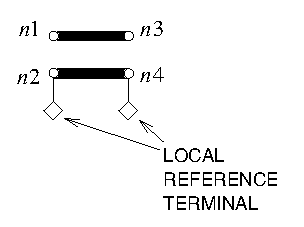
\includegraphics[scale=1.0]{tlinp4_multi.eps}}
\caption{\label{tlinp4:multi:model}Multi section model of a transmission line.}
\end{figure}
%
This model has two local reference terminals. An example netlist is:
\begin{verbatim}
l:1 n1 0 n3 ref1 z0=50 length=5mm
.ref "ref1"
\end{verbatim}
%%%%%%%%%%%%%%%%%
Here terminals `0' and `ref1' are the local reference terminals of the element. Terminal `0' is the global ground.  However `ref1' is a second local reference terminal of the element and either it or another terminal in the same local reference group must be specified as a reference terminal.  Here `ref1' is identified as a local reference terminal. (or a suitable terminal).  Another suitable example of a circuit would be
\begin{verbatim}
vsource 2 0 vac = 1 f = 5GHz
r:1 2 n1 r=50
r:2 0 n2 r=2
tlinp4:1 n1 n2 n3 n4 z0=50 length=5mm
r:3 n2 r=5
r:4 n4 5 r=100
r:5 n4 5 r=10
.ref 5
\end{verbatim}
tlinp4 above corresponds to Figure \ref{tlinp4:multi:model}. \\[0.2in]
\texttt{nsect} $>$ 0.\\[0.1in]
When  \texttt{nsect}, the number of sections, is a positive integer the transmission line is approximated using \texttt{nsect} sections. The model is shown in Figure \ref{tlinp4:section:model}.
\begin{figure}[h]
\centerline{Model with \texttt{nsect} $>$ 0.}
\centerline{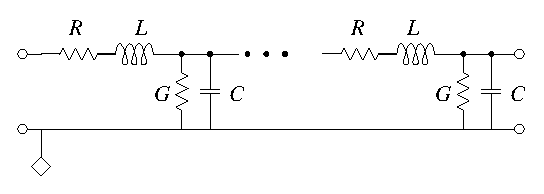
\includegraphics[scale=1.0]{tlinp4_sections.eps}} \caption{Multi section model of a transmission line.\label{tlinp4:section:model}}
\end{figure}
With respect to the terminal numbers in Figure \ref{tlinp4:multi:model}, terminals `n2' and `n4' must be the same terminal.
The sectional model is used in both the time domain and frequency domain.  Each series \emph{R} and inductance \emph{L} is modeled as a single \texttt{L} element. Each shunt \emph{G} and capacitance \emph{C} is modeled as a single \texttt{C} element. This is indicated in   Figure \ref{tlinp4:sectionb:model}
%\newline
\begin{figure}[h]
\centerline{Model with \texttt{nsect} $>$ 0.}
\centerline{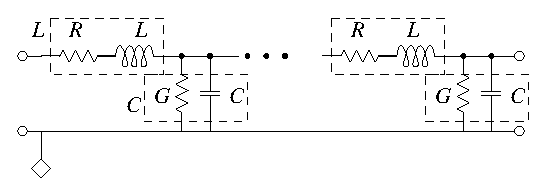
\includegraphics[scale=1.0]{tlinp4_sectionsb.eps}} \caption{Multi section model of a transmission line showing pairs of primitives each modeled by a single element.\label{tlinp4:sectionb:model}}
\end{figure}
The RLGC parameters of the model are calculated as follows.  (Note that R and L are noted as R$_{DC}$ and L$_{DC}$ in the skin effect section).
\begin{eqnarray}
\label{deltax} 
\Delta x = l/nsect
\end{eqnarray}
%
\begin{eqnarray}
\label{alpha} 
\alpha _f  = \left( {\alpha *0.11512925} \right)*\sqrt {{{f_{opt} } \over {f_{scale} }}} 
\end{eqnarray}
If \emph{f$_{opt}$} or \emph{f$_{scale}$} is not given or is 0 then $\alpha _f  = \left( {\alpha *0.11512925} \right)$
%
\begin{eqnarray}
\label{C} 
C = {{\sqrt k } \over {\left| {Z_0 } \right|*c_0 }}*\Delta x
\end{eqnarray}
%
\begin{eqnarray}
\label{L} 
L = \left| {Z_0 } \right|^2 *C
\end{eqnarray}
%
\begin{eqnarray}
\label{R} 
R = 2*\alpha _f *\left| {Z_0 } \right|*\Delta x
\end{eqnarray}
%
\begin{eqnarray}
\label{G} 
G = \tan d*2\pi *f_{opt} *C
\end{eqnarray}
If \emph{tand} or \emph{f$_{opt}$} is not given or is 0 then \emph{G=1*10$^{-10}$}
\newline
\myThickLine
\textit{Use of the skin effect:}
\newline
Setting of the \emph{fmax} parameter denotes the desire to use skin effect.  If \emph{fmax} is left out, the model behaves exactly as described above.  If skin effect modeling is desired, \emph{fmax} should be set to the maximum frequency at which the user expects the model to be valid.  Eg.  If the user is working at frequencies no higher then 10 GHz setting \emph{fmax} to 10e9 would be sufficient.  Setting \emph{fmax} to lower than the desired frequency will result in reduced accuracy.  Note if alpha is set to 0 (ideal conductors) then the skin effect will appear not to have any effect because by definition the model will have zero series resistance.  If fmax is not included, the transmission line subsections will be modeled as shown in Figure \ref{element_noskin}
\begin{figure}[h]
\centerline{Model with no skin effect}
\centerline{\includegraphics[scale=.7]{element_noskin.eps}} \caption{Transmission line subsection with skin effect not included
\label{element_noskin}}
\end{figure}
\vfill\eject
\begin{figure}[h]
\centerline{Model with skin effect}
\centerline{\includegraphics[scale=.8]{element_skin.eps}} \caption{Transmission line subsection with skin effect included
\label{element_skin}}
\end{figure}
\hspace*{\fill}
%
If skin effect is included the series resistance is modeled using a R-L stack as shown in Figure \ref{element_skin}.  The series \emph{R} and \emph{L} values are shown below for simplicity
\begin{eqnarray}
\label{Rseries} 
R = C_1 *R_{DC} *\left( {\sqrt {10} } \right)^m 
\end{eqnarray}
\begin{eqnarray}
\label{Lseries} 
L = C_2 *{{L_{DC} } \over {\left( {\sqrt {10} } \right)^m }}
\end{eqnarray}

\noindent\emph{R$_{DC}$} and \emph{L$_{DC}$} are the \emph{R} and \emph{L} values as calculated without skin effects as shown in (\ref{R}) and (\ref{L}).

The constants C$_1$ and C$_2$ are constants that are chosen based on the \emph{fmax} term, similarly the number of branches required, indexed by the \emph{m} variable, is chosen based on \emph{fmax} and will not exceed 9.  The table of values for C$_1$ and C$_2$ and m is shown in Table \ref{constants_table}.

 Sqrt(10) is chosen as the factor that will increase the resistance and decrease the inductance.  This value was picked experimentally such that after 1 MHz each additional branch (noted by the \emph{m} variable) makes the model valid for another decade of frequency.  As such the value of m$_{max}$ is found by consideration of fmax.  Eg. If fmax=10 MHz then m$_{max}$=2, if fmax=100 Mhz then m$_{max}$=3.
 \newline
\begin{table}[h]
\begin{center}
\begin{tabular}{|c|c|c|c|}
\hline
   fmax (Hz)   &C$_1$&C$_2$&m$_{max}$\\
\hline
   fmax $<$ 10    & 1 & 1& 0 \\
\hline
   fmax $<$ 10$^6$    & 1.32 & 1.68& 1 \\
\hline
   fmax $<$ 10$^7$    & 1.42 & 1.94& 2 \\
\hline
   fmax $<$ 10$^8$    & 1.45 & 2.03& 3 \\
\hline
   fmax $<$ 10$^9$    & 1.457 & 2.06& 4 \\
\hline
   fmax $<$ 10$^{10}$    & 1.461 & 2.07& 5 \\
\hline
   fmax $<$ 10$^{11}$    & 1.465 & 2.08& 6 \\
\hline
   fmax $<$ 10$^{12}$    & 1.4676 & 2.087& 7 \\
\hline
   fmax $<$ 10$^{13}$    & 1.4681 & 2.092& 8 \\
\hline
   fmax $<$ 10$^{14}$    & 1.4685 & 2.095& 9 \\
\hline
\end{tabular}
\caption{\label{constants_table}\emph{fmax} dependent model constants}
\end{center}
\end{table}
\newline
\textit{Derivation of Model Constants : }
\newline

The model constant C$_1$ was calculated such that at DC the parallel combination of all the (R) resistances are equal to R$_{DC}$ since the inductors are shorted at DC.  C$_2$ is somewhat more complicated but it is solved for iteratively by equating the low frequency phase of the skin effect R L with the low frequency phase of the R$_{DC}$ and L$_{DC}$ circuit in Figure\ref{element_noskin}. These can both be solved for based on the number of branches required.

Since the skin effect on a conductor can be thought of as the conductor being made of concentric shells.  At low frequencies all the shells carry currents and so the resistance seen is a DC resistance R$_{DC}$ in the model.  As frequency increases the inner shells turn off causing the DC resistance to increase and the internal inductance to decrease.
%%%%%%%%%%%%%%%%
\myThickLine
Example of Transient Analysis (.TRAN2) Fixed times steps, time-stepping nonlinear analysis.\\
netlist file: tlinp4.net:
\begin{verbatim}
* Transient tlinp4 test
.options f0 = 9e9
.tran2 tstop = 1e-9 tstep = .002e-9
vsource:v2 202 0 vdc= -6. vac= 5. f= f0 phase=90
resistor:rs 1 202 r=75.
tlinp4:t1  1 0 2 0
+ z0mag=75.00 nsect=1 length=978.57e-6 k=7 tand=.01 fscale=1.e10 alpha=1. fmax=1e10
resistor:rl 2 0  r=75.
.options gnuplot
.out plot term 1 vt in "tlinp4.1.tran"
.out plot term 2 vt in "tlinp4.2.tran"
.end
\end{verbatim}
The output log file is
\begin{verbatim}
**********  fREEDA 1.3 running on Wed Apr 29 11:13:35 2009  **********


   *** Parsing input netlist ...

   *** Expanding subcircuits ... done.

   *** Initializing and Expanding Elements ... done.

   *** Checking reference terminals ... done.

   *** Starting analysis ...

-----------------------------------------------------------------------------
   Matrix size = 13
   Matrix nnz = 47
   Using line search method.
   Nonlinear analysis tolerance (ftol) = 6.12865e-06
   Maximum number of nonlinear iterations per time-point (maxit) = 250
   Using Lee and Lee's quasi-Newton updates.
   --- Starting transient simulation ...

   Number of nonlinear state variables: 0
-----------------------------------------------------------------------------
   |  Step  |    Time (s)  |   Residual   |  Recent Max   |     Max      |
-----------------------------------------------------------------------------
   |      0 | 0.000000e+00 | 0.000000e+00 | 0.000000e+00  | 0.000000e+00 |
   |    200 | 4.000000e-10 | 0.000000e+00 | 0.000000e+00  | 0.000000e+00 |
   |    400 | 8.000000e-10 | 0.000000e+00 | 0.000000e+00  | 0.000000e+00 |
   --- Maximum Residual: 0
-----------------------------------------------------------------------------

 Plotting output file: tlinp4.1.tran.
 Plotting output file: tlinp4.2.tran.

**************  fREEDA 1.3 stopping on Wed Apr 29 11:13:35 2009  ***********
\end{verbatim}


\centerline{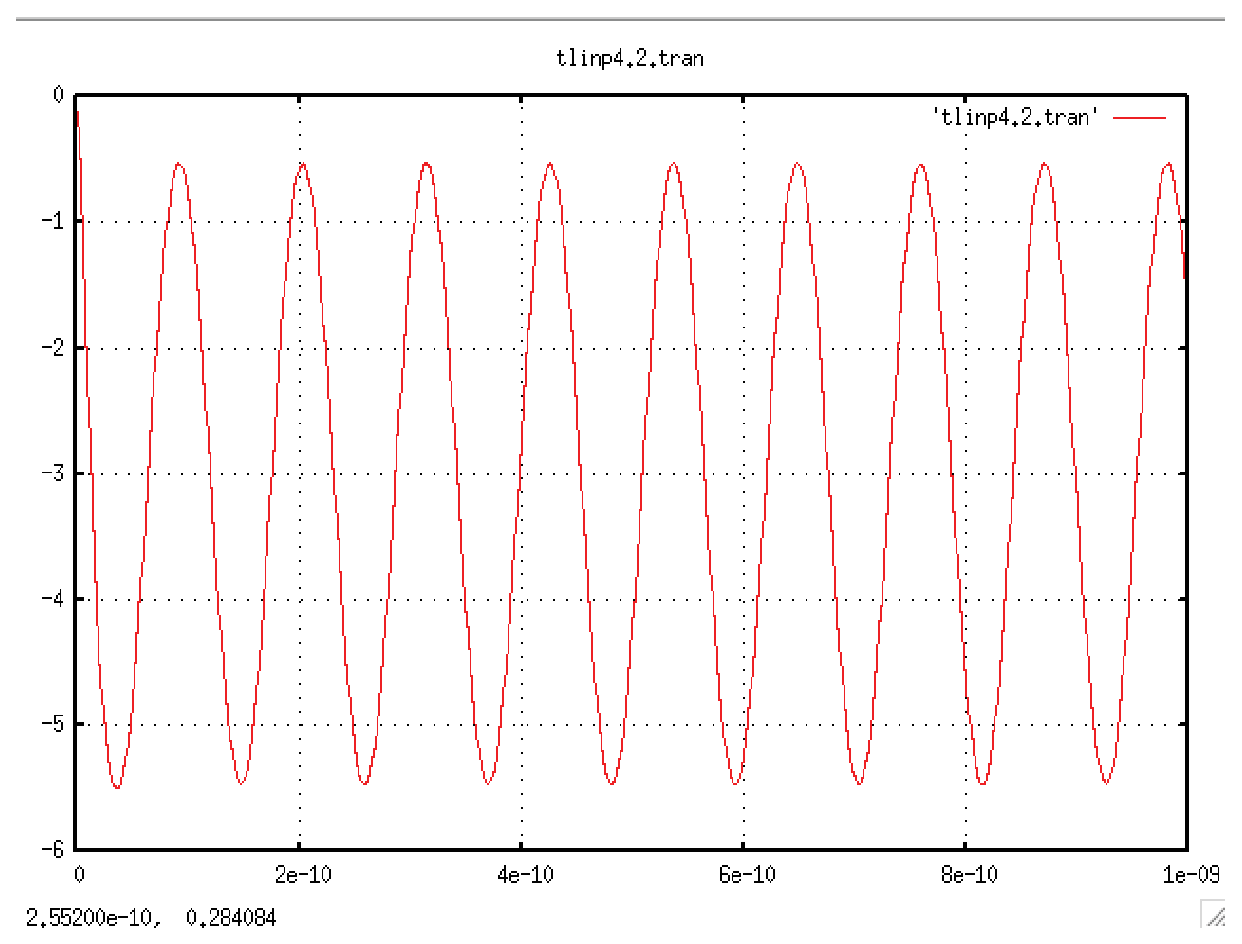
\includegraphics[width=3in]{tlinp4.2.tran.eps}}
~
\myThickLine
Example of Transient Analysis using Convolution (.SVTR).\\
In this example the transmission line is calculated in the frequency domain and convolution analysis is used to convert the model into an impulse response used directly in transient analysis.\\
netlist file: tlinp4\_conv.net:
\begin{verbatim}
* Transient tlinp4 test. Convolution is used
.options f0 = 9e9
.svtr tstop = 1e-9 tstep = .0002e-9
vsource:v2 202 0 vdc= -6. vac= 5. f= f0 phase=90
resistor:rs 1 202 r=75.
tlinp4:t1  1 0 2 ref2
+ z0mag=75.00 length=978.57e-6 k=7 tand=.01 fscale=1.e10 alpha=1. fmax=1e10
resistor:r3 2 ref2  r=75.
open:1 2 ref2
.ref "ref2"
.options gnuplot
.out plot element "open:1" 0 ut in "tlinp4.2.svtr"
.end
\end{verbatim}
Note that in convolution analysis augmentation elements are used to provide the proper interface between the linear and nonlinear partitions of the circuit analyzed in the time-domain and frequency-domain. As well all linear elements internal to the linear circuit partition care not available. Consequently the voltages at terminals of linear elements are not available and the voltages at the terminals of nonlinear elements are modified by the augmentation circuit. Voltages and currents must be obtained from nonlinear elements (using \texttt{ut} and \texttt{it}). Additional nonlinear elements can be introduced using the \texttt{open} element which is treated as tough it is a nonlinear element.  So to get the voltage at a particular terminal either an existing nonlinear element can be exploited or an \texttt{open} element introduced. The voltage determine the voltage (ut) of that element is used.  In the above \texttt{element "open:1" 0 ut} indicates that the first (the zero'th) \texttt{ut} voltage of the element \texttt{open:1} is pushed on the stack.\\[0.1in]
The output log file follows:
\begin{verbatim}
**********  fREEDA 1.3 running on Wed Apr 29 11:31:42 2009  **********


   *** Parsing input netlist ...

   *** Expanding subcircuits ... done.

   *** Initializing and Expanding Elements ... done.

   *** Checking reference terminals ... done.

   *** Starting analysis ...

-----------------------------------------------------------------------------
   *** State Variable-Based Transient Analysis ***
-----------------------------------------------------------------------------

   n_samples = 1792
   Frequency step = 2.43902e+09 Hz
   Maximum frequency = 2.49756e+12 Hz
   Number of time steps = 5001

   --- Building Msv(f) ...
   Number of state variables = 2
   --- Converting Msv to the time domain ...

   Warning: Last 35 samples impulse contribution: 1.72 %

   Warning: Last 35 samples impulse contribution: 25.01 %

   Warning: Last 35 samples impulse contribution: 25.01 %

   Warning: Last 35 samples impulse contribution: 5.57 %
   --- Starting transient simulation ...

   Using line search method.
   Nonlinear analysis tolerance (ftol) = 6.12865e-06
   Maximum number of nonlinear iterations per time-point (maxit) = 250
   Using Lee and Lee's quasi-Newton updates.
-----------------------------------------------------------------------------
   |   Step   |    Time (s)    |   Residual (V)   |
-----------------------------------------------------------------------------
   |     100  |  2.000000e-11  |  1.333760e-14    |
   |     200  |  4.000000e-11  |  1.959041e-14    |
   |     300  |  6.000000e-11  |  2.203514e-14    |
   |     400  |  8.000000e-11  |  2.237927e-14    |
   |     500  |  1.000000e-10  |  2.250559e-14    |
   |     600  |  1.200000e-10  |  2.388845e-14    |
   |     700  |  1.400000e-10  |  2.675828e-14    |
   |     800  |  1.600000e-10  |  3.062149e-14    |
   |     900  |  1.800000e-10  |  3.157902e-14    |
   |    1000  |  2.000000e-10  |  3.168229e-14    |
   |    1100  |  2.200000e-10  |  3.193301e-14    |
   |    1200  |  2.400000e-10  |  3.328842e-14    |
   |    1300  |  2.600000e-10  |  3.689638e-14    |
   |    1400  |  2.800000e-10  |  3.872710e-14    |
   |    1500  |  3.000000e-10  |  3.905102e-14    |
   |    1600  |  3.200000e-10  |  3.912686e-14    |
   |    1700  |  3.400000e-10  |  3.974990e-14    |
   |    1800  |  3.600000e-10  |  4.197954e-14    |
   |    1900  |  3.800000e-10  |  4.506976e-14    |
   |    2000  |  4.000000e-10  |  4.588288e-14    |
   |    2100  |  4.200000e-10  |  4.596716e-14    |
   |    2200  |  4.400000e-10  |  4.612777e-14    |
   |    2300  |  4.600000e-10  |  4.749799e-14    |
   |    2400  |  4.800000e-10  |  4.974311e-14    |
   |    2500  |  5.000000e-10  |  5.141199e-14    |
   |    2600  |  5.200000e-10  |  5.173273e-14    |
   |    2700  |  5.400000e-10  |  5.176453e-14    |
   |    2800  |  5.600000e-10  |  5.215110e-14    |
   |    2900  |  5.800000e-10  |  5.358540e-14    |
   |    3000  |  6.000000e-10  |  5.559405e-14    |
   |    3100  |  6.200000e-10  |  5.638657e-14    |
   |    3200  |  6.400000e-10  |  5.647929e-14    |
   |    3300  |  6.600000e-10  |  5.658068e-14    |
   |    3400  |  6.800000e-10  |  5.732690e-14    |
   |    3500  |  7.000000e-10  |  5.913543e-14    |
   |    3600  |  7.200000e-10  |  6.068913e-14    |
   |    3700  |  7.400000e-10  |  6.108066e-14    |
   |    3800  |  7.600000e-10  |  6.111576e-14    |
   |    3900  |  7.800000e-10  |  6.129309e-14    |
   |    4000  |  8.000000e-10  |  6.279185e-14    |
   |    4100  |  8.200000e-10  |  6.440435e-14    |
   |    4200  |  8.400000e-10  |  6.524856e-14    |
   |    4300  |  8.600000e-10  |  6.533710e-14    |
   |    4400  |  8.800000e-10  |  6.541732e-14    |
   |    4500  |  9.000000e-10  |  6.602423e-14    |
   |    4600  |  9.200000e-10  |  6.745446e-14    |
   |    4700  |  9.400000e-10  |  6.890652e-14    |
   |    4800  |  9.600000e-10  |  6.934587e-14    |
   |    4900  |  9.800000e-10  |  6.937813e-14    |
   |    5000  |  1.000000e-09  |  6.954280e-14    |
-----------------------------------------------------------------------------

   --- Residual: 6.95428e-14
   --- Writing output vectors ...
 Plotting output file: tlinp4.2.svtr.

**************  fREEDA 1.3 stopping on Wed Apr 29 11:31:50 2009  ***********
\end{verbatim}
%%%%%%%%%%%%%%%%%%%%%
\hspace*{\fill}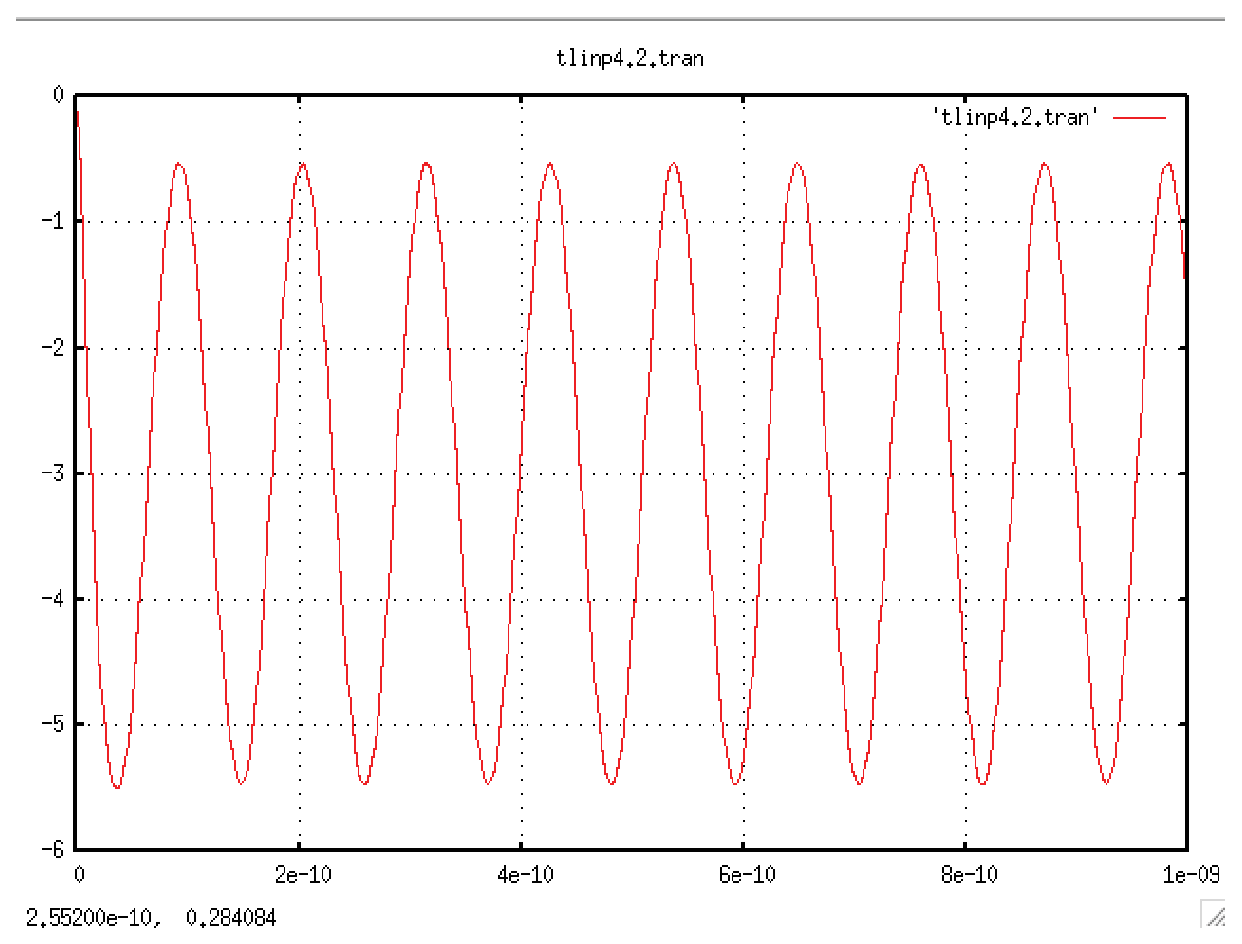
\includegraphics[width=3in]{tlinp4.2.svtr.eps}\hfill
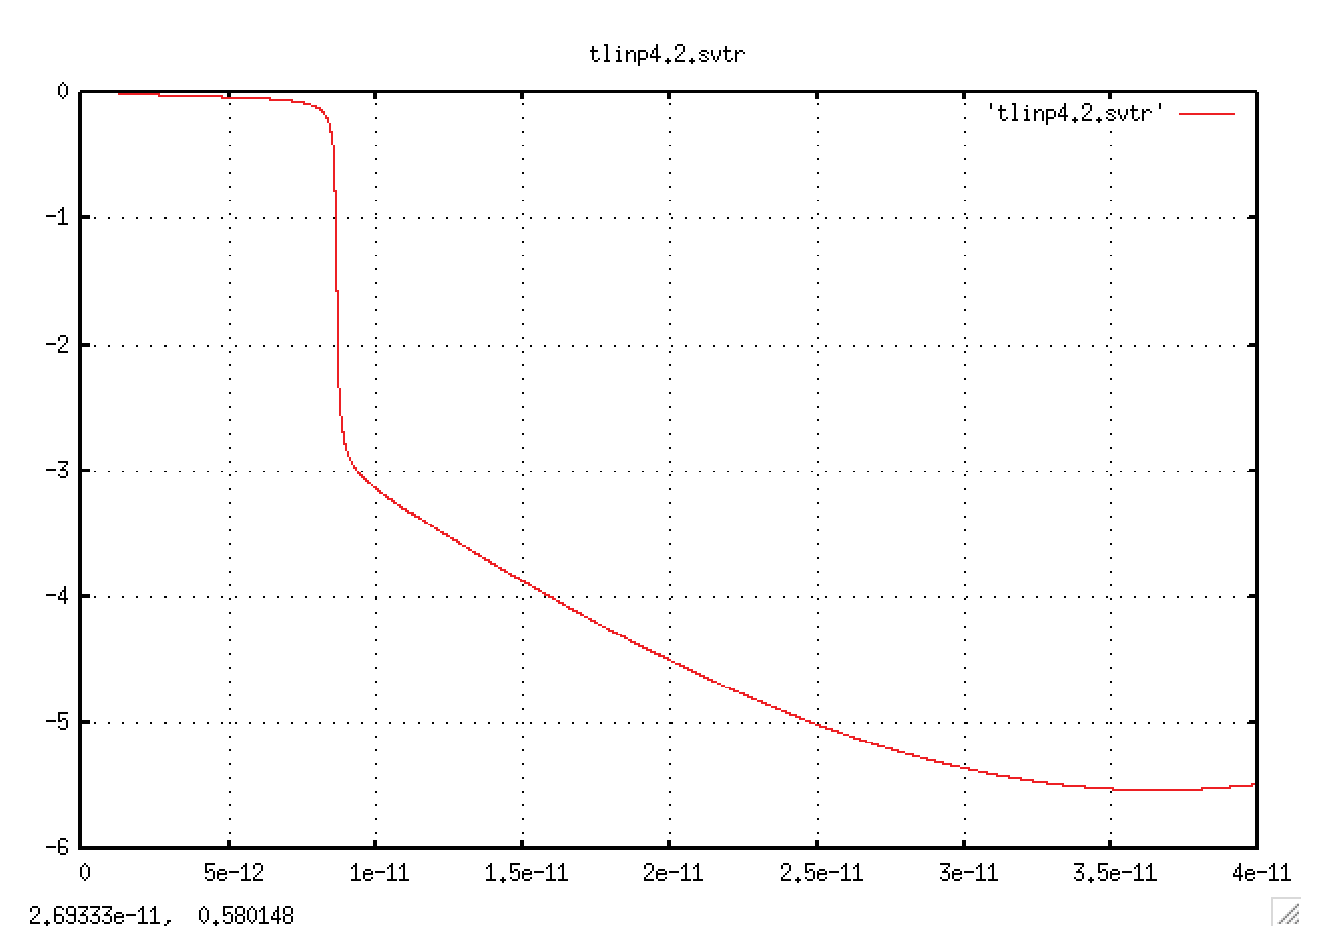
\includegraphics[width=3in]{tlinp4.2.svtr.z.eps}\hspace*{\fill}
~
\myThickLine
Example of AC Analysis using single subsection calculations.\\
netlist file: tlinp4AC.net:
\begin{verbatim}
* AC tlinp4 test
.ac start = 1 stop = 20GHz n_freqs=10000
vsource:v2 202 0  vac= 5
resistor:rs 1 202 r=75.
tlinp4:t1  1 0 2 ref2
+ z0mag=75.00 length=0.03 k=7 tand=.1 fscale=1.e10 alpha=1 fmax=20e9
resistor:rl 2 ref2  r=75.
.ref "ref2"
.options gnuplot
* Get the magnitude of the voltage at terminal 2. This is with respect to ref2
.options preamble1="set term x11 font 'helvetica,13';
set xlabel 'FREQUENCY (GHz)'; set ylabel 'MAGNITUDE (VOLTS)"
.out plot term 2 vf mag 1e-9 scalex preamble1 in "tlinp4.2.mag"
* Get the phase of the voltage at terminal 2. This is with respect to ref2
* prinphase gets the principal phase as opposed to the continuous phase.
.options preamble2="set term x11 font 'helvetica,13';
set xlabel 'FREQUENCY (GHz)'; set ylabel 'phase (DEGREES)"
.out plot term 2 vf prinphase 1e-9 scalex rad2deg preamble2 in "tlinp4.2.phase"
.end
\end{verbatim}

The output log file is:
\begin{verbatim}
**********  fREEDA 1.3 running on Wed Apr 29 11:46:15 2009  **********

   *** Parsing input netlist ...

   *** Expanding subcircuits ... done.

   *** Initializing and Expanding Elements ... done.

   *** Checking reference terminals ... done.

   *** Starting analysis ...

-----------------------------------------------------------------------------
   *** AC Analysis ***
-----------------------------------------------------------------------------

   Frequency step = 2.0002e+06 Hz
   --- Writing output vectors ...
 Plotting output file: tlinp4.2.mag.
 Plotting output file: tlinp4.2.phase.
**************  fREEDA 1.3 stopping on Wed Apr 29 11:46:15 2009  ***********
\end{verbatim}
And the results are: 
\newline
\emph{With Skin effect : }
\newline
%\hspace*{\fill}
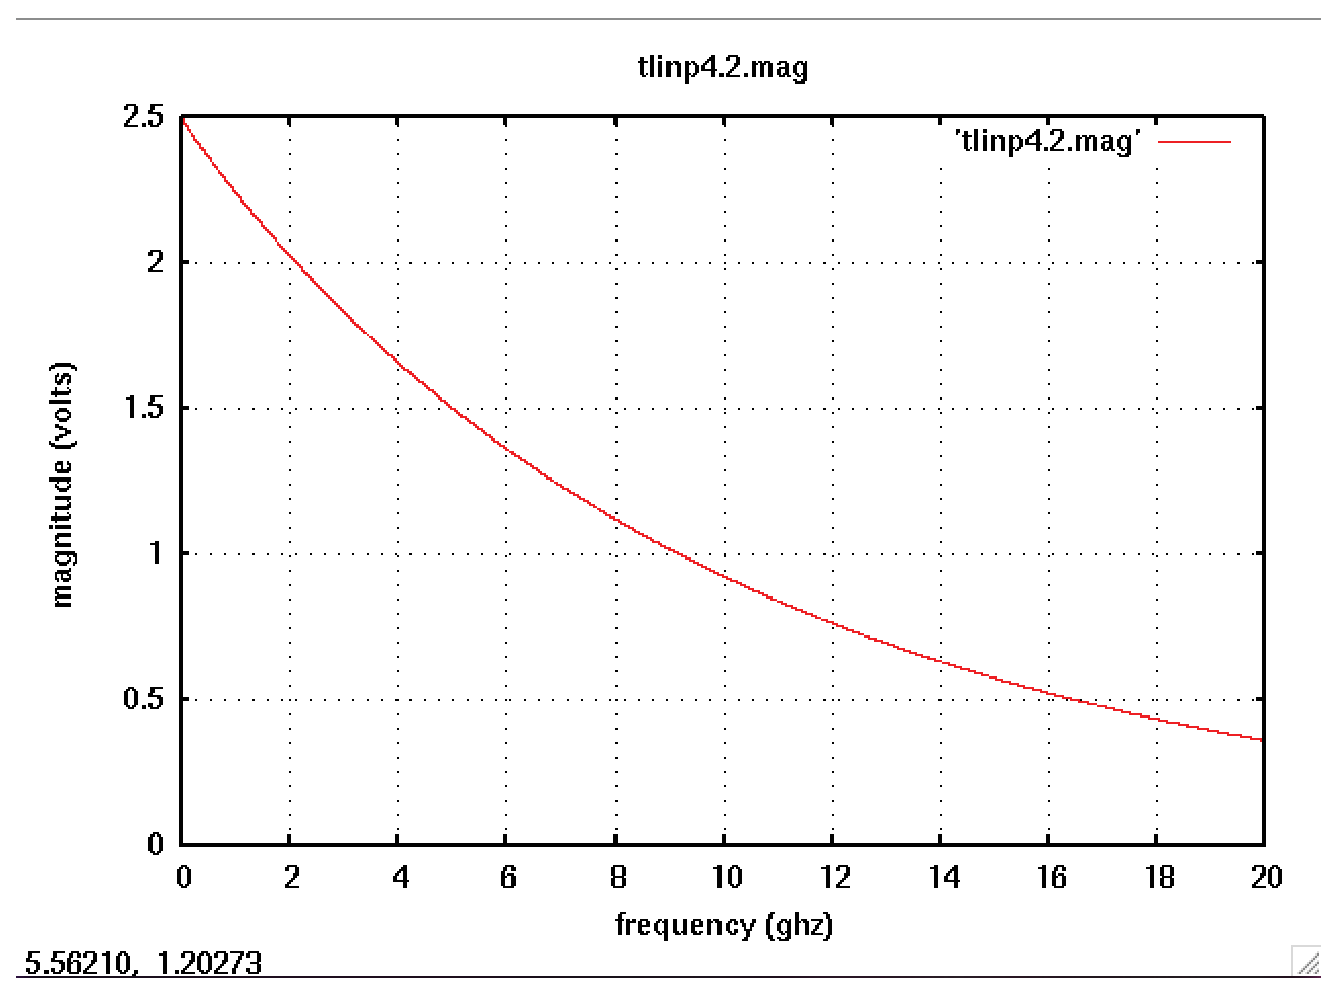
\includegraphics[width=3in]{tlinp4.2.mag.eps}\hfill
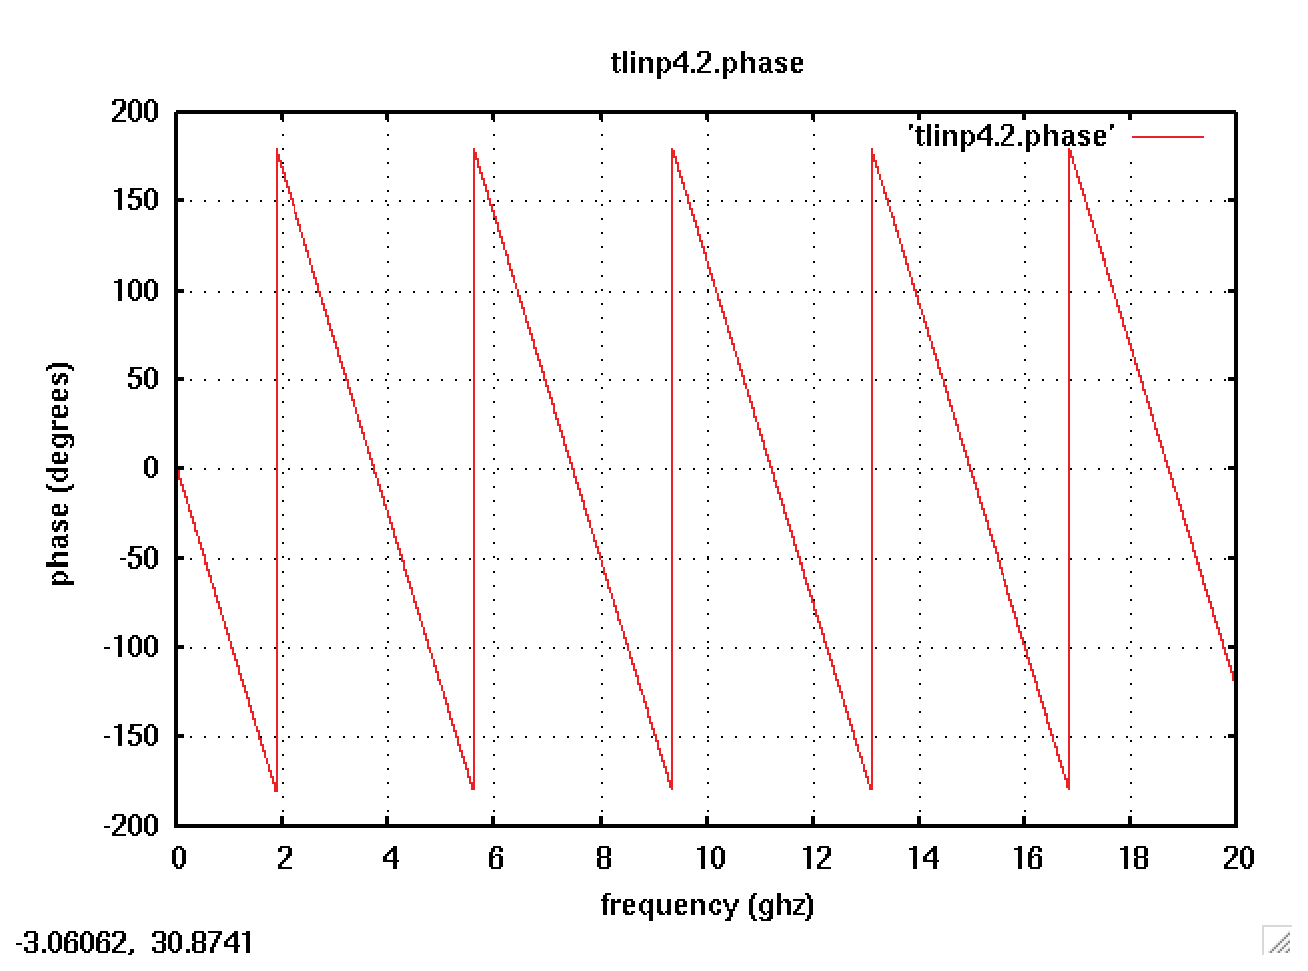
\includegraphics[width=3in]{tlinp4.2.phase.eps}\hspace*{\fill}
~\\
\emph{Without Skin effect : }
\newline
%\hspace*{\fill}
\includegraphics[width=3in]{tlinp4.2.mag_noskin.eps}\hfill
\includegraphics[width=3in]{tlinp4.2.phase_noskin.eps}\hspace*{\fill}
~\\
Notice how the plots appear to be the exact same with or without skin effect, this is to be expected because this is only a one subsection model of the transmission line and as such is a very poor approximation.  The series inductor, \emph{L$_{DC}$}, dominates at the higher frequencies and begins to look like an open circuit, as such the output voltage shown in the plot moves exponentially towards zero.  See the next section for the example of a multiple subsection simulation.
\myThickLine
\newline
Example of AC Analysis using a multi subsection approximation\\
netlist file: tlinp4AC2.net:
\begin{verbatim}
* AC tlinp4 test
.ac start = 1 stop = 10GHz n_freqs=10000
vsource:v2 202 ref2  vac= 5
resistor:rs 1 202 r=75.
tlinp4:t1  1 ref2 2 ref2
+ z0mag=50.00 length=.03 k=7 tand=.1 nsect=20 alpha=1 fmax=2e10
resistor:rl 2 ref2  r=75.
.ref "ref2"
.options gnuplot
* Get the magnitude of the voltage at terminal 2. This is with respect to ref2
.options preamble1="set term x11 font 'helvetica,13';
set xlabel 'FREQUENCY (GHz)'; set ylabel 'MAGNITUDE (VOLTS)"
.out plot term 2 vf mag 1e-9 scalex preamble1 in "tlinp4.2.mag"
* Get the phase of the voltage at terminal 2. This is with respect to ref2
* prinphase gets the principal phase as opposed to the continuous phase.
.options preamble2="set term x11 font 'helvetica,13';
set xlabel 'FREQUENCY (GHz)'; set ylabel 'phase (DEGREES)"
.out plot term 2 vf prinphase 1e-9 scalex rad2deg preamble2 in "tlinp4.2.phase"
.end
\end{verbatim}

The output log file is:
\begin{verbatim}
**********  fREEDA 1.3 running on Wed Apr 29 13:37:27 2009  **********


   *** Parsing input netlist ...

   *** Expanding subcircuits ... done.

   *** Initializing and Expanding Elements ... done.

   *** Checking reference terminals ... done.

   *** Starting analysis ...

-----------------------------------------------------------------------------
   *** AC Analysis ***
-----------------------------------------------------------------------------

   Frequency step = 1.0001e+06 Hz
   --- Writing output vectors ...
 Plotting output file: tlinp4.2.mag.
 Plotting output file: tlinp4.2.phase.

**************  fREEDA 1.3 stopping on Wed Apr 29 13:37:27 2009  ***********
\end{verbatim}
And the results are: 
\newline
\emph{With Skin effect : }
\newline
%\hspace*{\fill}
\includegraphics[width=3in]{tlinp4.2.mag_nsect_skin.eps}\hfill
\includegraphics[width=3in]{tlinp4.2.phase_nsect_skin.eps}\hspace*{\fill}
~\\
\emph{Without Skin effect : }
\newline
%\hspace*{\fill}
\includegraphics[width=3in]{tlinp4.2.mag_nsect_noskin.eps}\hfill
\includegraphics[width=3in]{tlinp4.2.phase_nsect_noskin.eps}\hspace*{\fill}
~\\
In the above graphs notice how the plots without skin effect lack any significant attenuation at higher frequencies while the skin effect model attenuates more at the higher frequencies.  These plots perhaps best illustrate the use of the skin effect model.

This time we are using a 20 subsection approximation, it is a much better approximation than the single subsection approximation above.  In the graphs below, standing waves can be seen with peaks corresponding to the phase wrapping in the phase graph.  This is because the model is using LC pairs and as such it is a resonance structure.
\myThickLine
\textit{Version:}\\
2009.04.029 (2009 April 29) \\
% Credits
\myThickLine
\medskip
\textit{Credits:}\\
\begin{tabular}{l l l l}
Name & Affiliation & Date & Links \\
Carlos E. Christofferson, Mete Ozkar & NC State University & Sept 2000 & 
\includegraphics[width=1in]{logo.eps}  \\
cechrist@ieee.org & & & www.ncsu.edu    \\\\
Michael Steer & NC State University & April 2008 & 
\includegraphics[width=1in]{logo.eps}  \\
mbsteer@ieee.org & & & www.ncsu.edu    \\\\
Austin Samples & NC State University & April 2009 & 
\includegraphics[width=1in]{logo.eps}  \\
atsample@ncsu.edu & & & www.ncsu.edu    \\
\end{tabular}
\end{document}